%-----------------------------------------------------------------------------
%
%               Template for sigplanconf LaTeX Class
%
% Name:         sigplanconf-template.tex
%
% Purpose:      A template for sigplanconf.cls, which is a LaTeX 2e class
%               file for SIGPLAN conference proceedings.
%
% Guide:        Refer to "Author's Guide to the ACM SIGPLAN Class,"
%               sigplanconf-guide.pdf
%
% Author:       Paul C. Anagnostopoulos
%               Windfall Software
%               978 371-2316
%               paul@windfall.com
%
% Created:      15 February 2005
%
%-----------------------------------------------------------------------------


\documentclass[10pt, preprint]{sigplanconf}

% The following \documentclass options may be useful:

% preprint      Remove this option only once the paper is in final form.
% 10pt          To set in 10-point type instead of 9-point.
% 11pt          To set in 11-point type instead of 9-point.
% authoryear    To obtain author/year citation style instead of numeric.

\usepackage{amsmath}
\usepackage{graphicx}

\begin{document}

\special{papersize=8.5in,11in}
\setlength{\pdfpageheight}{\paperheight}
\setlength{\pdfpagewidth}{\paperwidth}

\conferenceinfo{SPLASH '15}{Oct 25--30, 2015, Pittsburgh, Pennsylvania, USA} 
\copyrightyear{2015} 
\copyrightdata{978-1-nnnn-nnnn-n/yy/mm} %D What goes here?
\doi{nnnnnnn.nnnnnnn} 								 %D and here?

% Uncomment one of the following two, if you are not going for the 
% traditional copyright transfer agreement.

%\exclusivelicense                % ACM gets exclusive license to publish, 
                                  % you retain copyright

%\permissiontopublish             % ACM gets nonexclusive license to publish
                                  % (paid open-access papers, 
                                  % short abstracts)

\titlebanner{DRAFT -- DO NOT DISTRIBUTE}        % These are ignored unless
\preprintfooter{A literate program family approach to scientific software}   % 'preprint' option specified.

\title{Learning to Cook 'ware}
\subtitle{A Family Approach} %D Something about prog families?

\authorinfo{Daniel Szymczak}
           {McMaster University}
           {szymczdm@mcmaster.ca}
\authorinfo{Spencer Smith\and Jacques Carette}
           {McMaster University}
           {smiths at mcmaster.ca/carette at mcmaster.ca}

\maketitle

\begin{abstract}
  This is where we will put the abstract of our paper. It will be
  super-fantastic and make all the reviewers think that this should not only be
  accepted, but most definitely published. %D Going to need to work on this
\end{abstract}

\category{CR-number}{subcategory}{third-level}

% general terms are not compulsory anymore, 
% you may leave them out
\terms
term1, term2 %D What goes here?

\keywords Program families, generative programming, documentation, scientific
computing, literate programming %D Should anything else go here?

\section{Introduction} 

Scientific computing (SC) was the first application of computers. It is still
used today for a wide variety of tasks: constructing mathematical models,
performing quantitative analyses, creating simulations, solving scientific
problems, etc. SC software has been developed for increasingly safety and
security critical systems (nuclear reactor simulation, satellite
guidance%D MORE EXAMPLES)
) as well as predictive
systems. %D Change the next bit about applications, pick better examples that
         %fit with the theme: nuclear / avionics / automotive
It has applications including (but not limited to) predicting weather patterns
and natural disasters, and simulating economic fluctuations. As such, it is an
incredibly important part of an increasing number of industries
today.%D and can be seen as a third mode of science which complements experimentation and theory.

%D Removed something about earthquake prediction as an example.
In the medical, nuclear power, aerospace, automotive, and manufacturing fields
there are many safety critical systems in play. With each system, there is the
possibility of a catastrophic failure endangering lives. It is incredibly
important then to have some means of certifying and assuring the quality of each
software system. As Smith et al. \cite{SmithEtAl2013} stated
``Certification of Scientific Computing (SC) software is official recognition by
an authority or regulatory body that the software is fit for its intended use.''
These regulatory bodies determine certain certification standards that must be
met for a system to become recognized as certified. One example of a
certification standard is the Canadian Standards Association (CSA) requirements
for quality assurance of scientific software for nuclear power plants.

The main goal of software certification is to ``... systematically determine,
based on the principles of science, engineering, and measurement theory, whether
a software product satisfies accepted, well-defined and measurable criteria''
\cite{HHLMWW}. As such, certification would not only involve analyzing the code
systematically and rigorously, but also analyzing the
documentation. Essentially, this means the software must be both valid and
verifiable, reliable, usable, maintainable, reusable, understandable, and
reproducible. %D Verification involves ensuring that the software is ``solving
              %the equations right'', whereas validation requires ensuring that
              %the software is ``solving the right equations''\cite{Roache1998}.

Developing certifiable software can end up being a much more involved process
than developing uncertified software: it takes more money, time, and effort on
the part of developers to produce. These increased costs lead to reluctance from
practitioners to develop certifiable software \cite{Roache1998}. However, in
our %D my?
opinion, cost is not the only contributing factor for the developers. As it
stands in the field, scientists seem to prefer a more agile development process
\cite{Segal2008}. Typically this would lead to problems maintaining the
documentation, meaning that not all aspects of the software would be traceable
through the design process and making certification more difficult (if not
impossible).

Given proper methods and tools, scientists would be able to follow a more
structured approach (while capitalizing on frequent feedback and course
correction) to meet documentation requirements for certification as well as
improve their overall productivity. This is where our work comes in: our goal is
to eat our cake and have it too.  We want to improve the qualities
(verifiability, reliability, understandability etc.) and at the same time
improve performance.  Moreover, we want to improve developer productivity; save
time and money on SC software development, certification and
re-certification. To accomplish this we need to do the following:

\begin{enumerate}
\item Remove duplication between software artifacts for scientific computing
  software \cite{WilsonEtAl2013}
\item Provide complete traceability between all artifacts
\end{enumerate}

To achieve the above goals, we propose the following:

\begin{enumerate}
\item Provide methods, tools and techniques to support developing scientific
  software using a literate process
\item Use ideas from software product lines, or program families
\item Use code generation
\end{enumerate}

Section \ref{sec:background} will give a more in-depth look at SC software,
specifically focusing on SC software quality (including historical attempts to
improve quality), the program family approach, and literate programming. Section
\ref{sec:what} focuses on what a literate family approach can achieve,
specifically related to software certification; domain knowledge capture;
simplification, reusability, and portability; optimization; verification; and
how it can incorporate non-functional requirements as well as
functional. Finally, section \ref{sec:concluding} will provide a few concluding
remarks.

\section{Background} \label{sec:background}

Throughout the history of computing, specifically scientific computing, there
have been many challenges towards assuring the quality of software. Many
attempts have been made (some successful, others not) at improving the software
quality. In this section we will discuss those attempts and challenges, as well
as introduce the ideas behind our proposed approach.

\subsection{Challenges for SC Software Quality} \label{subsec:challenges}

SC software has certain characteristics which create challenges for its
development. We will not discuss them all in depth, however, those of interest
to us are the approximation, unknown solution, technique, input output, and
modification challenges as described by Yu \cite{Yu2011}.

The \textit{approximation challenge} is a challenge to SC software's
reliability. Since real numbers are approximated by floating point numbers on
computers, round off and truncation errors can be introduced to a SC software
system during computation steps. While any single step may introduce a very
small error, they can compound quickly and become unmanageable.

The \textit{unknown solution challenge} is another challenge to SC software's
reliability. This challenge arises when SC programs are used to solve problems
with unknown true solutions, i.e. there are very limited test cases with known
solutions. As such, the accuracy and precision of the software can be hard (if
not impossible) to judge.

The \textit{technique selection challenge} is a challenge that comes up often
when dealing with continuous mathematical equations. Since these cannot be
solved directly (due to computers being discrete), some technique must be chosen
which can produce a solution which is ``good enough'' for the user. Choosing the
technique to use is typically left to domain experts as each technique will
(not) satisfy certain non-functional requirements.

The \textit{input output} challenge impacts the usability of SC software and
typically comes up where considerable amounts of input data are used in the
production of large volumes of output. The main issue in this case is the
complicated nature of the input data and the output, leading developers to
recreate existing library routines (slightly modified) to deal with the
nature of the input and output.

Finally, the \textit{modification challenge} tends to come up as requirements
change. As SC software is used at the forefront of scientific knowledge, there
can be a high frequency of requirements changes. As changing requirements can
mean completely modified systems, it poses a problem for scientists: commercial
software can be difficult/expensive to modify and noncommercial programs are not
often flexible enough to change.

\subsection{History of Attempts to Improve Quality} \label{subsec:history}

SC software has not seen many focused attempts at improving software
quality. Most attempts at improving software quality have been aimed at a
broader target than SC specifically. However, many of the methods used have been
useful to SC software. Yu \cite{Yu2011} addresses the issue in-depth, but we
will give a brief overview.

The object-orientation (OO) approach aims to increase software quality through
the use of several mechanisms. \textit{Encapsulation} ensures information hiding
\cite{Parnas1972a} by keeping information hidden from the classes that do not
require it. \textit{Inheritance} is useful in the OO approach, but not
necessarily when applied to SC as many SC problems do not deal with a
hierarchical structure. \textit{Polymorphism} can improve reusability by, for
example, allowing algorithms to be bound at runtime (though the use of abstract
classes). However, for SC software, the algorithm being solved is typically
known ahead of time and thus a general program using different algorithms is not
necessarily useful.

Agile methods, on the other hand, are one of the most prevalent approaches used
by software engineers. It is useful in the context of SC software as it allows
for flexibility in dealing with unpredictably changing requirements, on the flip
side, if the requirements are fairly stable there is no real benefit to using
agile methods.  However, many practitioners of SC may claim that their
requirements are not stable. This may be true for individual programs, but if
we think of the exercise as developing a family of related programs, then the
requirements are stable. The experimentation performed by SC developers is
an exercise in modifying the variabilities within a program family.

A program family approach is meant to improve reusability. As the program family
is reused and retested, it is likely that any defects will be discovered, thus
improving reliability. Developing a program family is a general, plan-driven
approach. Where agile methods dealt with unpredictably changing requirements,
the program family approach is tailored toward projects with stable or
predictably changing requirements. The program family is designed such that each
member solves a small set of problems, and we will discuss it in more depth in
Section \ref{subsec:program}. %D Mention maintainability in sebsec:program.

There are several other techniques for improving SC software quality. The use of
\textit{libraries}, for one, is a fairly standard technique used in many areas
of software development. However, in SC software, libraries can be cumbersome or
difficult to use due to the variety of their
subroutines. \textit{Component-based development (CBD)} is similar to the
library approach, but the components that are being reused are not restricted to
subroutines, and CBD suggests techniques for the development of reusable
components.

A \textit{problem solving environment (PSE)} is similar to both libraries and
CBD, however, it is much more involved. A PSE provides all of the facilities
necessary for solving a class of problems. This includes (semi-)automatic
solution method selection, advanced solution methods, and the means to include
novel solutions. Combining PSEs and libraries can help avoid the difficulties of
using libraries independently \cite{RiceAndBoisvert1996}. PSEs have already been
used for SC for years, with major examples being Matlab and Maple.

Another technique is \textit{aspect-oriented programming (AOP)}. It is similar
to the OO approach mentioned above in that the main focus is separating
concerns, however, AOP deals with cross-cutting concerns of a system (ex:
logging). Aspects modularize supporting functions and isolate them from the
business logic of the main program.

\textit{Generic programming} is a technique for developing reusable
software. Generic programming looks at an algorithm and determines the
commonalities between similar implementations of it. From there, a single,
generic algorithm is created (through the use of abstractions) which will be
able to cover many concrete implementations.

\textit{Generative programming} is used for automatically creating members of
program families. Given a requirements specification, generative programming can
produce highly customized and optimized products on demand. The product is
manufactured using reusable implementation components and specific configuration
knowledge.

Finally, \textit{design patterns} are solutions to recurring problems in
software design. Each pattern is both general and reusable. Essentially, design
patterns are templates for solving problems (that can occur in many different
situations), and are typically found in OO design. As such, design patterns can
be used in SC in certain cases where the OO approach is taken.

As far as we know, there has not been an empirical study to measure the
effectiveness of any of the above approaches for SC software.

\subsection{Program Family Approach} \label{subsec:program}

In the previous section, we introduced the idea of a program family approach. To
re-iterate: the program family approach should be used in projects with stable,
or predictably changing, requirements. The program family approach is reusable,
reliable, and easily maintainable.

Reusability of program families is enforced by design. If the product were not
reusable, there would be no reason to undertake a program family
approach. Reliability stems from the reuse of the common core of the program
family; defects are more likely to be found. Finally, since the core assets of
the program family are managed together, it is easier to maintain.

In a program family, each member is not a general purpose program. The family
members each solve a specific (small) set of problems. This can lead to
increased usability, as there is no need to configure a general purpose program
for a specific problem.

Determining how or when to apply the program family approach can be
difficult. However, Weiss \cite{Weiss} proposed a strategy which relies on three
assumptions (phrased as hypotheses) which aid in determining whether a domain is
suitable for the program family approach. The hypotheses are as follows:

\begin{itemize}
\item \textit{The Redevelopment Hypothesis}: Most software development consists
  of a majority of redevelopment. Existing software systems are modified to
  create new variations as opposed to entirely new software systems. In most
  cases, these variations are more alike than different from each other.
\item \textit{The Oracle Hypothesis}: Changes to a piece of software over its
  lifetime can be predicted. Specifically, necessary types of variations of a
  system can be predicted.
\item \textit{The Organizational Hypothesis}: The software may be organized in
  such a way that predicted changes of one type can be made independently of
  other types of changes. Essentially, changing at most a few modules in the
  system for any given type of change.
\end{itemize}

Many SC programs can be developed as families because they adhere to these
hypotheses. With respect to the redevelopment hypothesis, SC software that
performs simulations, for example, typically has several of its own
assumptions. If these assumptions are modified, then it is likely that the
software can now perform a different (hopefully useful) simulation. The same
applies to any SC software which solve problems in similar ways: there is reuse
of common functionality so it would necessarily be redeveloped in other
situations.

Many SC software adhere to the oracle hypothesis since they are equations that
model scientific theories which have been studied over many, many years. The
theories are stable, so any change to the software is predictable. Changes to
the computational design are generally known ahead of time or can be estimated
by the domain specialists (scientists).

The organizational hypothesis holds for SC software as well, but perhaps not as
strongly as the other two (yet). As we mentioned, a major area of change are the
underlying assumptions for programs. These assumption changes for the models are
not often strongly dependent, thus few modules would need to be changed to
modify the software. However, there is typically a strong connection between
algorithms and data structures in SC software, but separating the data
structures from the algorithms is not impossible \cite{Berti2000a, ElSheikhEtAl2004}.

%D - many examples where reuse has not been achieved -- Give a recent one.

\subsection{Literate Programming} \label{subsec:literate}

Literate programming (LP) is a programming methodology introduced by Knuth
\cite{Knuth1984}. The main idea behind it is writing programs in a way that
allows us to explain (to humans) what we want the computer to do, as opposed to
simply telling the computer what to do. There is a focus on ordering the
material to promote better human understanding.

In a literate program, the documentation and code are kept together in one
source. The program is an interconnected web of code pieces, presented in any
sequence. As part of the development process, the algorithms used in literate
programming are broken down into small, easy to understand parts (known as
``sections'' \cite{Knuth1984} or ``chunks'' \cite{Johnson1997}) which are
explained, documented, and implemented in a more intuitive order for better
understanding.

To extract the source code or documentation from the literate program,
certain processes must be run. To get working source code, the \textit{tangle}
process would be run, essentially extracting the code from the literate document
and reordering it into an appropriate structure for the computer to
understand.  To get a human-readable document, the \textit{weaving}
process must be run to extract and typeset the documentation.

By adhering to the LP methodology, a literate program ends up with documentation
that is expertly written and of publishable quality. The code also ends up being
incredibly well documented and high-quality. There are several examples of SC
programs being written in LP style, and two that stand out are VNODE-LP
\cite{Nedialkov2006} and ``Physically Based Rendering: From Theory to
Implementation'' \cite{PharrAndHumphreys2004} (a literate program / textbook).

\section{What is Possible with a Literate Family Approach} \label{sec:what}

A literate family approach is a combination of literate programming, program
families, and code generation. The main goals of this approach (mentioned
earlier) are to improve qualities (verifiability, reliability, etc.) while
improving performance and productivity to save money and time on software
development, certification, and re-certification.

To achieve these goals, we begin by taking a literate approach to
software development. For our purposes we will be focusing on SC software, but
there are many potential domains of application for the literate family
approach. The literate approach helps to break down the problems into easily
explained chunks, capturing domain knowledge and ensuring high-quality code and
documentation.

As we will be looking at SC software, we also take a program family approach to
find commonalities between similar implementations of algorithms. Analyzing
commonalities allows us to determine the core versus the configuration of an
algorithm. Once the core has been determined, we intend to use code generation
to implement the program family (and its members) in a simple and
straightforward manner. Since the code will be generated from the knowledge
captured in the LP-style chunks (which we sometimes refer to as
\textit{ingredients}) according to a \textit{recipe}, the documentation for each
family member can also be generated from a
recipe. %D maybe change the next line.
Having a family of programs with high-quality documentation for little cost to
developers would be an enormous benefit and would aid in certifying the family
of programs.

%D Family meal example here to set things up?

%D - this is the discussion section - give advantages and then use examples to
% illustrate D Should I just introduce the sections following or actually get
% into the examples before they start?

\subsection{Software Certification} \label{subsec:software}

To certify software there is a need for high-quality
documentation. This documentation needs to be created without impeding the work
of scientists. One of the major problems with creating documentation for SC
software stems from the modification challenge (Section
\ref{subsec:challenges}). As the requirements change, the documentation must be
updated. The further scientists are into a project, the greater the effect a
change of requirements will have on the documentation, leading to
maintainability and traceability issues.

The cost of making changes to the documentation should be reasonable. The best
way to keep costs low is to ensure the traceability of the
documentation. Traceability allows the developers to track which areas of a
project will be affected by a change, thus allowing them to ensure that those
areas are updated accordingly.

Depending on the regulatory body and set of standards for certification, many
types of documents can be required. Our approach aims to generate all of these
documents alongside the code, accounting for any changes made. As the changes
will affect ingredients and those ingredients will be used to generate the
 documentation, there is a guarantee that changes will propogate throughout all
  of the documents. The following are examples of ``default'' documents that 
we want to create (we assume software engineers will be familiar with most, 
if not all, of these):

\begin{itemize}
\item Problem Statement: A description of the problem to be solved, essentially
  summarizing the purpose of the software. There should be no mention of how the
  problem is to be solved.
\item Development Plan: An overview of the development process and
  infrastructure. This should cover the documents to be created, which templates
  (if any) will be followed, internal processes to be employed, coding
  standards, and other details relevant to how the software will be developed.
\item Requirements Specification: The desired functions and qualities of the
  software should be documented herein. The requirements should cover
  functionality, goals, context, design constraints, expected performance, and
  any other quality attributes of the software.
\item Verification and Validation plan: Documents how the documentation
  artifacts will be shown to be internally correct (verification) as well as how
  to ensure that the right problem has been solved (validation).
\item Design Specification: How will the requirements be realized? Document the
  software architecture and a detailed design of the modules/interfaces to be
  used. Can be thought of as a programmer's manual for maintenance.
\item Code: Implementation of the design specification.
\item Verification and Validation Report: Summarize the steps taken for
  performing verification and validation (this should mirror the V \& V plan
  from above) and include any testing results.
\item User Manual: Full instructions on how the software is to be used,
  beginning with installation instructions and proceeding through detailed
  examples of the program's use.
\end{itemize}

The documents listed above share non-trivial amounts of information, which is
where traceability comes into play. To make any changes to the
documentation, there must be some way to determine how a change will affect
\textbf{all} of the documents.

This is especially important for (re-) certification, as the documents must be 
consistent.

In the context of re-certification, if a program was developed using the literate 
family approach and some changes needed to be made, updating the 
documentation and submitting it for re-certification would be completely trivial. 
All documentation would be generated from the newly modified ingredients, 
according to their existing recipes.

On another note, if a document standard were to be changed during the 
development cycle, it would not necessitate re-writing the entire document. All
 of the information in the ingredients would remain intact, only the recipe 
 would need to be changed to accomodate the new standard.

\textbf{An example would be good here.  We could use fuelpin example.}

\subsection{Knowledge Capture} \label{subsec:knowledge}

Capturing scientific knowledge is essential to implementing effective SC
software families. Many formulae are commonly shared between a variety of 
different practical applications. %D Being able to capture not only the relevant
%D equations, but also the meaning behind them improves the quality
%D I'm not sure where I'm going with this intro -- needs edits.

As an example, consider the conservation of thermal energy equation:
\begin{equation}
CONSERVATION EQN.
\end{equation}
This equation is used for thermal analysis of fuel pins, %previous example
but is also used in applications like solar water heating tanks \cite{}. 
%D Elaborate

\begin{figure}
	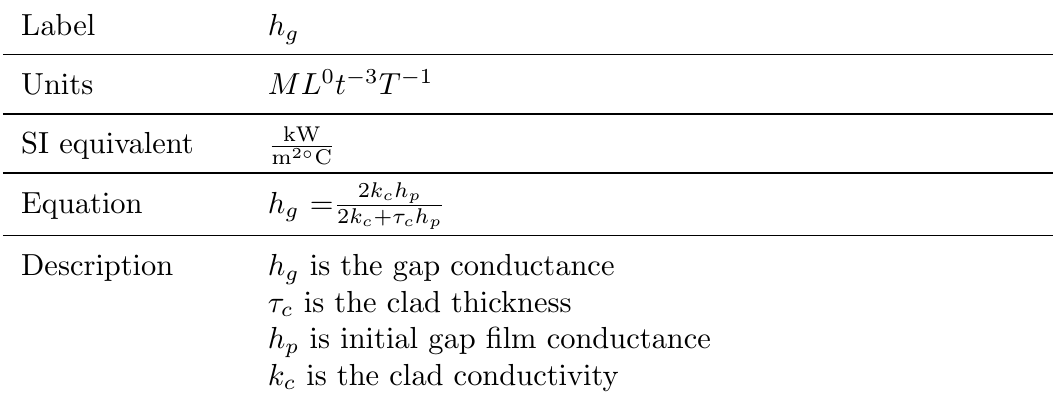
\includegraphics[width=8.5cm]{figures/h_g}
	\caption{SRS data definition of $h_g$}
\label{fig:h_g}
\end{figure}	

\begin{figure}
	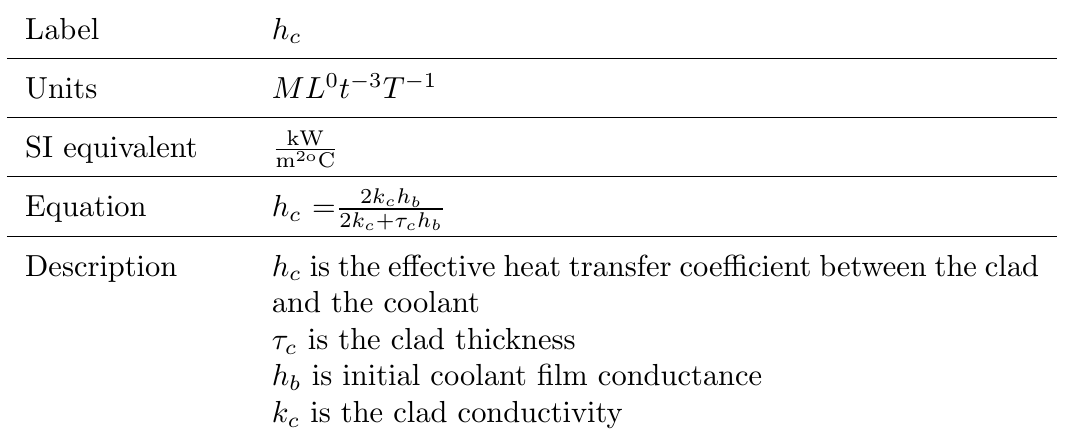
\includegraphics[width=8.5cm]{figures/h_c}
	\caption{SRS data definition of $h_c$}
	\label{fig:h_c}
\end{figure}	

From the fuel pin example (again), if we look at the equation for the gap
conductance from Figure~\ref{fig:h_g} and the equation for heat transfer 
coefficient between clad and coolant from Figure~\ref{fig:h_c}, 
we can see that there is common knowledge necessary for calculating both 
of these values (i.e. $k_{c}$ and $\tau_c$). Now, rather than redefining the 
common terms in these equations in each document where they appear, 
we consider each unique symbol as its own ingredient. 
Both $h_g$ and $h_c$ are also ingredients, thus they need only
reference the ingredients used in their equations to express all of the
requisite knowledge for implementation.

For the documentation related to $h_g$ and $h_c$, the recipe for each document
will fill in the appropriate details related to any and all symbols that appear
in the equations, which can be seen in the ``Description'' section of 
Figures~\ref{fig:h_g}~\&~\ref{fig:h_c}. Now if we needed to update the 
description of any symbol, we would simply update it in one place (its
ingredient) and the recipe would handle propagating the change through all
of the documentation and code.

From the above example it should be clear that this approach allows for the
development of a library of artifacts (ingredients) related to SC software
that capture domain knowledge and can be reused in multiple contexts while
remaining maintainable and traceable. Another benefit of creating such a library
of artifacts is it would combine many sources of knowledge while keeping
the notations and terminology consistent and ensuring that all underlying 
assumptions are well documented.

%Build a library of artifacts that can be reused in many different contexts -
%example of “Commonality Analysis for a Family of Material Models”
%(FamilyOfMaterialModels - not yet published - in mmsc repos) - the section
%on the purpose of the document (Section 1.1) discusses how the documentation
%combines various sources and uses a consistent notation and terminology

\subsection{``Everything should be made as simple as possible, but not
  simpler.'' (Einstein quote)}  \label{subsec:everything}

Currently there exist many powerful, general commercial programs for solving
problems using the finite element method. However, they are not often used
to develop new ``widgets'' because of the cost and complexity of doing so.
As it stands, engineers often have to resort to building prototypes and testing
them instead of performing simulations due to a lack of tools that can assist
with their exact set of problems.

A literate family approach could change that by generating members according
to the needs of the engineers. For example, if an engineer is designing parts 
for strength, they could have a general stress analysis program. This program 
could be 3D or specialized for plane stress or strain, depending on which 
assumption would be the most appropriate. The program could even be specialized
further, to be customized to the parameterized shape of the part that the
engineer is interested in. This new specialized program can expose only the 
degrees of freedom that the engineer can change (ex. material properties or
specific dimensions of the part), making the entire simulation process simpler
and safer.


\subsection{Optimization} \label{subsec:optimization}

- Connect optimization with analysis.  Optimization requires running multiple
analysis cases.  Code generation can be used to build an efficient model that
has just what is needed, and no more.  As the optimization searches the design
space, new models can be generated.  - An optimization problem for a part where
the shape and constitutive equation are degrees of freedom, cite family of
material models (SmithMcCutchanAndCarette2014)

\textbf{An example would be good here.  Unfortunately, I do not have one that
  has previously been worked out.}

\subsection{Verification} \label{subsec:verification}

When it comes to verification, requirements documents typically include
so-called ``sanity'' checks that can be reused throughout subsequent phases
of development. For instance, the requirement would state conservation of mass
or that lengths are always positive. The former would be used to test the output
and the latter to guard against some invalid inputs.

With a literate family approach, these sanity checks can be ensured by the 
knowledge capture mechanism. Each ingredient can maintain its own sanity
checks and incorporate them into the final system to make sure that all inputs
and outputs (including intermediaries) are valid.

- computational variability testing, from Yu (2011), FEM example - usual to do
grid refinement tests - same order of interpolation, but more points - code
generation allows for increases in the order of interpolation, for the same grid
- Yu discusses in section 6.3 of her thesis

\subsection{Incorporating Non-Functional Requirements in a decision support
  system for selecting the best design options} \label{subsec:incorporating}

A literate family approach will necessarily be able to create multiple family
members that can solve the same problem in slightly different ways (ex.
different algorithm choices), so how should a decision be made between them?
Traditionally when designing software, this is where the engineers would compare
the non-functional requirements of the system to the different implementations,
then make a decision based on how those requirements are being satisfied.

The decision making process can be performed through the literate family
approach by using the Analytic Hierarchy Process (AHP)~\cite{Smith2006}. AHP is
a method for comparing attributes by using a ratio scale to prioritize these
attributes. The priorities are then determined by a series of pair-wise 
comparisons between attributes. AHP has had great success in decision analysis,
and as such it is the method we have chosen for ranking non-functional 
requirements.

Once we have decided on the relative rankings of our different non-functional
requirements, we can analyze the family members that solve our problem and
select the one which does the best job of incorporating the non-functional 
requirements in their priority order.

%D Show example of AHP table?


\section{Concluding Remarks} \label{sec:concluding}

Concluding remarks.

\section*{References}

\bibliographystyle{abbrvnat}
\bibliography{LitProgFamDevInSC}

\appendix
\section{Appendix Title}

This is the text of the appendix, if you need one.

\acks

Acknowledgments, if needed.

\end{document}

%                       Revision History
%                       -------- -------
%  Date         Person  Ver.    Change
%  ----         ------  ----    ------

%  2013.06.29   TU      0.1--4  comments on permission/copyright notices

